\problemset{Теория вероятностей и математическая статистика}
\problemset{Индивидуальное домашнее задание №1}

% Команда ниже задает "название" или слово, которое будет
% отображаться вместо proof или "доказательство"
% поскольку у нас в ИДЗ задачи - то нужно слово "Решение"
\renewcommand*{\proofname}{Решение}

%%%%%%%%%%%%%% ЗАДАНИЕ №1 %%%%%%%%%%%%%%
%% Условие задания №1
\begin{problem}
Из 35 книг, среди которых трехтомник А.С.Пушкина, выбирается наугад 18 и выставляется на полку. Определить вероятность того, что все три книги тома попадут на полку.\\
\end{problem}

%% Решение задания №1
\begin{proof}
Для начала определим множество исходов $\Omega$. Ясно, что в данном случае элементарным событием будет $ \omega_i $ = \{"данные 18 книг (из 35) выставлены на полку"\}. То есть $ \omega_i $ есть конкретное сочетание 18 книг из 35.\\Тогда очевидно, что:
\[ \#\Omega = \binom{35}{18} = \frac{35!}{18!\cdot\left(35-18\right)!} \]
Теперь определим событие $ A $. Подходят все элементарные события (сочетания 18 книг из 35), которые включают в себя книги трехтомника. А таких всего:
\[  \#A = \binom{3}{3}\cdot\binom{32}{15} = \frac{32!}{15!\cdot\left(32-15\right)!} \]

(тут учли, что были точно выбраны книги трехтомника и еще некоторые из оставшихся 32 книг)

Отсюда получаем, что вероятность наступления события $ A $ равна:
\[\frac{\#A}{\#\Omega} = \frac{32!}{15!\cdot17!}\cdot\frac{18!\cdot17!}{35!} = \frac{48}{385} \approx 0.1247 \]

{\it Ответ:} 0.1247
\end{proof}

%%%%%%%%%%%%%% ЗАДАНИЕ №2 %%%%%%%%%%%%%%
%% Условие задания №2
\begin{problem}
Прямые разбивают плоскость на полосы ширины 8. Определить вероятность того, то отрезок длинны 3, наугад брошенный на плоскость, не пересечет ни одной прямой.\\
\end{problem}

%% Решение задания №2
\begin{proof}
Ясно, что данная вероятностная задача относится к разделу задач на геометрическое определение вероятности. 
Одним из ограничений геометрического определения вероятности является условие, накладываемое на множество исходов $ \Omega $. Хоть само множество бесконечно большое (его мощность бесконечна), но мера $ V_d $ множества $ \Omega $ в пространсве $ \Real^d$ конечна.

В условии задачи же под $ \Omega $ автор понимает всю плоскость, а её мера $ V_2 $ в пространсве $ \Real^2 $ бесконечна. Мы получили некорректную формулировку вероятностной задачи.

Попробуем переформулировать задачу.
Неважно, в какую именно часть плоскости будет брошен отрезок, он всегда попадет как минимум на одну полосу (поскольку полос бесконечно много). Причем неважно, на какую именно полосу попал отрезок, полосы одинаковые, плоскость в любой части выглядит одинаково. 

Это значит, что достаточно рассмотреть в качестве $ \Omega $ лишь одну полосу ширины 8, вероятность того, что отрезок пересечет эту полосу и будет являться искомой вероятностью.

При этом не важно, что ширина полосы равна 8, а длинна бесконечна, ведь полоса в любой части относительно длинны выглядит одинаково, неважно, упал отрезок ниже или выше, он все равно упал на полосу.

Нарисуем картинку для решения задачи (см. рис.1).
\begin{figure}
    \centering
    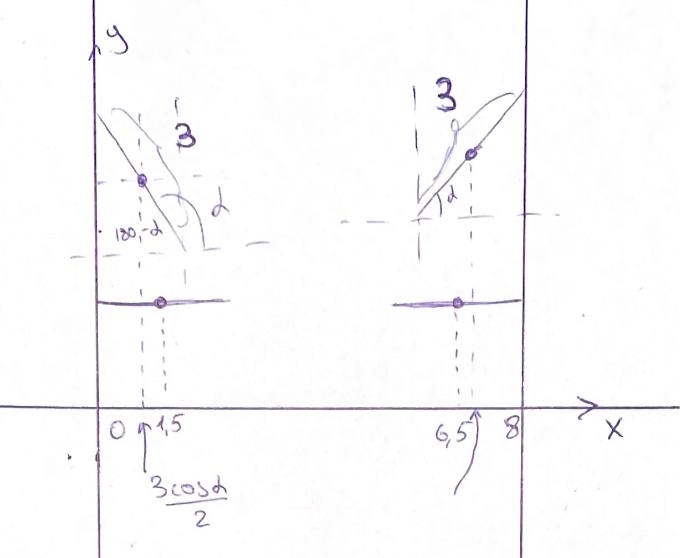
\includegraphics[width=0.5\linewidth]{1.jpg}
    \caption{}
    \label{fig:enter-label}
\end{figure}

Пусть $ x $ - это положение центра отрезка, а $ \alpha $ - угол между осью $ X $ и отрезком.\\
$ A =$ \{"отрезок не пересек ни одной прямой"\} - событие, вероятность которого нужно найти.\\
Соответственно $ 0\le x\le8 $ и $ 0\le\alpha\le\pi$.
Понятно, что при $ 1,5\le x\le6,5 $ угол может быть любым, а вот для остальных участков интервала на $ x $ и $ \alpha $ накладываются ограничения. Из рисунка видно, что чтобы отрезок не пересек прямую, нужно, чтобы:
\[
\begin{cases}
    x\ge\frac{3}{2}\cos{\alpha} 1.5, & \mbox{если } 0\le x < 1,5 \\
    x\le 8 - \frac{3}{2}\cos{\alpha}, & \mbox{если } 6,5 < x\le 8
\end{cases}
\]

Изобразим множества $ A $ и $ \Omega $ (см. рис.2).
\begin{figure}
    \centering
    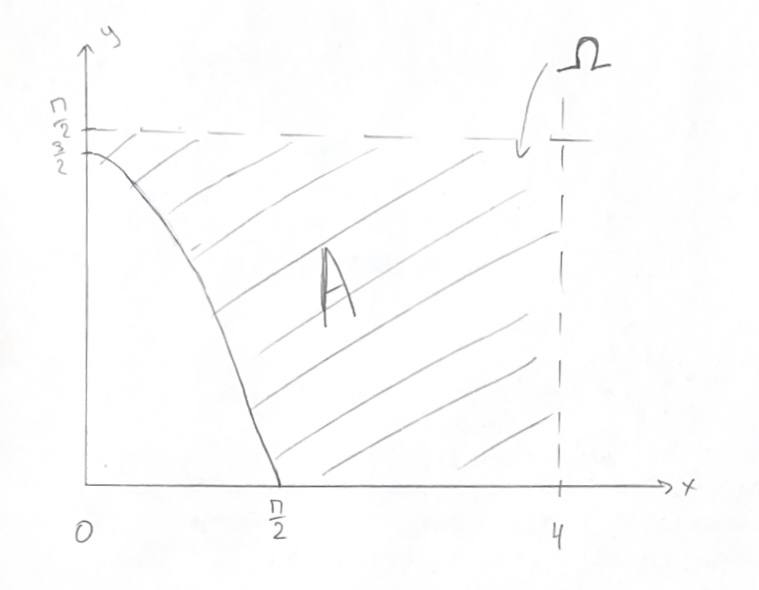
\includegraphics[width=0.5\linewidth]{2.jpg}
    \caption{}
    \label{fig:enter-label}
\end{figure}
Очевидно, что $ V_2\left(\Omega\right) = 8\pi$.\\
А вот меру $ A $ найдем вычитанием из меры (площади) $ \Omega $ мер (площадей) незаштрихованных уголков. Они, кстати, симметричны и площадь одного такого уголка можно найти как:

\[
\int\limits_0^{\pi/2} \frac{3}{2}\cos{\alpha} \, d\alpha = 1,5
\]
Тогда $ V_2\left(A\right) = 8\pi - 2\cdot 1,5 = 8\pi - 3$

Используя определение геометрической вероятности, находим, что:
\[
\Prob\left(A\right) = \frac{V_2\left(A\right)}{V_2\left(\Omega\right)} = \frac{8\pi - 3}{8\pi} = 1 - \frac{3}{8\pi} \approx 0.8806
\]
{\it Ответ:} 0.8806
\end{proof}

%%%%%%%%%%%%%% ЗАДАНИЕ №3 %%%%%%%%%%%%%%
%% Условие задания №3
\begin{problem}
В первой урне находится 8 белых и 8 красных шаров; во второй - 8 белых и 10 красных шаров; в третьей - 18 белых и 10 красных шаров. Наугад выбирают одну урну. Из неё достали 2 шара. Все оказались белыми. Определить вероятность того, что они из первой урны.\\
\end{problem}

%% Решение задания №3
\begin{proof}
Построим таблицу для определения ПГС.\\
Пусть $ H_1 $ = \{"Шары доставали из первой урны"\}. $ H_2 $ = \{"Шары доставали из второй урны"\}. $ H_3 $ = \{"Шары доставали из третьей урны"\}.\\
Событие $ A $ = \{"Из урны достали два белых шара"\}.\\
В итоге найти нам нужно вероятность $ H_1 $ при условии события $ A $.
\begin{center}
\begin{tabular}{ |c|c|c|c|c| } 
    \hline
    - & $ H_1 $ & $ H_2 $ & $ H_3 $ & $ \sum $\\ 
    \hline
    $\Prob\left(H_i\right)$ & $\frac{1}{3}$ & $\frac{1}{3}$ & $\frac{1}{3}$ & 1\\ 
    \hline
    $\Prob\left(A|H_i\right)$ & $\frac{8}{16}\cdot\frac{7}{15}$ & $\frac{8}{18}\cdot\frac{7}{17}$ & $\frac{18}{28}\cdot\frac{17}{27}$ & - \\ 
    \hline
\end{tabular}
\end{center}
Найдем вероятность события $ A $, используя формулу полной вероятности:
\[
\Prob\left(A\right) = \sum_{i=1}^3 \Prob\left(A|H_i\right)\cdot\Prob\left(H_i\right) = \frac{8}{16}\cdot\frac{7}{15}\cdot\frac{1}{3} + \frac{8}{18}\cdot\frac{7}{17}\cdot\frac{1}{3} + \frac{18}{28}\cdot\frac{17}{27}\cdot\frac{1}{3} = \frac{4397}{16065}
\]
Найдем вероятность $ H_1 $ используя формулу Байеса:
\[
\Prob\left(H_1|A\right) = \frac{\Prob\left(A|H_1\right)\cdot\Prob\left(H_1\right)}{\Prob\left(A\right)} = \frac{\frac{7}{30}\cdot\frac{1}{3}}{\frac{4397}{16065}} = \frac{2499}{8794} \approx 0.2842
\]
{\it Ответ:} 0.2842
\end{proof}

%%%%%%%%%%%%%% ЗАДАНИЕ №4 %%%%%%%%%%%%%%
%% Условие задания №4
\begin{problem}
Электростанция находится в городе А, из которого проведены ЛЭП в посёлки В и С. Кроме того посёлки В и С соеденены ЛЭП между собой и с посёлком D каждый. В результате урагана вероятность повреждения линий AB и AC равна 0.5, а линий BC, BD и CD - 0.3. Определить вероятность того, что электроснабжение посёлка D не будет нарушено.
\end{problem}

%% Решение задания №4
\begin{proof}
Для решения задачи нарисуем рисунок (см. рис.3).
\begin{figure}
    \centering
    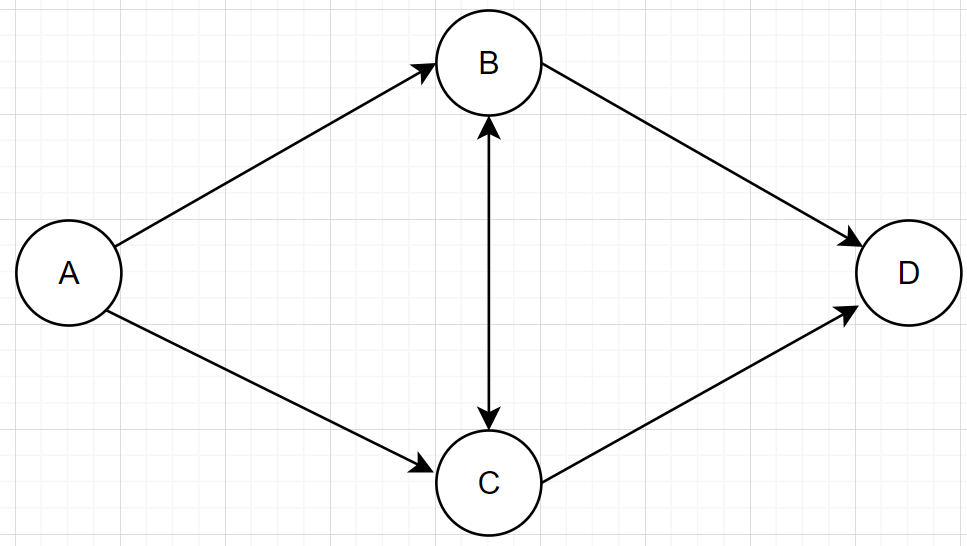
\includegraphics[width=0.5\linewidth]{3.png}
    \caption{}
    \label{fig:enter-label}
\end{figure}

Пусть событие $ A = $ \{"Электроснабжение посёлка D не будет нарушено"\}. Тогда, событие $ \neg A = $ \{"Электроснабжение посёлка D будет нарушено"\}. Понятно, что легче всего посчитать вероятность события $ \neg A $, тогда вероятность события $ A $ найдется как:
\[
\Prob\left(A\right) = 1 - \Prob\left(\neg A\right)
\]

Электроснабжение будет нарушено в четырех случаях:\\
1) Повредились линии AB и AC\\
2) Повредились линии BD и CD\\
3) Повредились линии AC, BC и BD\\
4) Повредились линии AВ, BC и СD\\
Любой из этих случаев приводит к нарушению электроснабжения.
То есть:
\[
\Prob\left(\neg A\right) = \Prob\left(1\cup 2\cup 3\cup 4\right) = \Prob\left(1\right) + \Prob\left(2\right) + \Prob\left(3\right) + \Prob\left(4\right)
\]
Где:
\begin{gather*}
    \Prob\left(1\right) = \Prob\left(AB\cap AC\right) = \Prob\left(AB\right)\cdot\Prob\left(AC\right) = 0.5\cdot 0.5 = 0.25\\
    \Prob\left(2\right) = \Prob\left(BD\cap CD\right) = \Prob\left(BD\right)\cdot\Prob\left(CD\right) = 0.3\cdot 0.3 = 0.09\\
    \Prob\left(3\right) = \Prob\left(AC\cap BC\cap BD\right) = \Prob\left(AC\right)\cdot\Prob\left(BC\right)\cdot\Prob\left(BD\right) = 0.5\cdot 0.3\cdot 0.3 = 0.045\\
    \Prob\left(4\right) = \Prob\left(AB\cap BC\cap CD\right) = \Prob\left(AB\right)\cdot\Prob\left(BC\right)\cdot\Prob\left(CD\right) = 0.5\cdot 0.3\cdot 0.3 = 0.045
\end{gather*}
Тут учли, что события \{"повреждена линия X"\} и \{"повреждена линия Y"\} независимые, следовательно вероятность их пересечения равна произведению вероятностей каждого из событий.
Итого $ \Prob\left(\neg A\right) = 0.25 + 0.09 + 0.045 + 0.045 = 0.43 $\\
Тогда $ \Prob\left(A\right) = 1 - \Prob\left(\neg A\right) = 1 - 0.43 = 0.57$

{\it Ответ:} 0.57
\end{proof}

%%%%%%%%%%%%%% ЗАДАНИЕ №5 %%%%%%%%%%%%%%
%% Условие задания №5
\begin{problem}
Вероятность успеха в схеме берунли равна $ \frac{1}{5} $. Проводится 2000 испытаний. Написать точную формулу и вычислить приближённо вероятность того, что число успехов равно 382.
\end{problem}

%% Решение задания №5
\begin{proof}
Воспользуемся формулой $ \Prob\left(\mu_n = k\right) = \binom{n}{k}\cdot p^k\cdot\left(1-p\right)^{n-k} $\\
Тогда $ \Prob\left(\mu_{2000} = 382\right) = \binom{2000}{382}\cdot 0.2^{382}\cdot 0.8^{1618} $\\
Поскольку проводится большое число испытаний, посчитаем вероятность приближенно.
$ n\cdot p = 2000\cdot\frac{1}{5} = 400 > 10 \Rightarrow $ воспользуемся схемой Муавра-Лапласа:
\[
P_n\left(k\right) \approx \frac{1}{\sqrt{np(1-p)}}\cdot\varphi(X_{n,k})
\]
Где $ \varphi(x) = \frac{1}{\sqrt{2\pi}}\cdot\exp{\left(-\frac{x^2}{2}\right)} $ и $ X_{n,k} = \frac{k - np}{\sqrt{np(1-p)}} $.

\begin{gather*}
    X_{2000, 382} = \frac{382 - 2000\cdot 0.2}{\sqrt{2000\cdot 0.2\cdot 0.8}} \approx -1.00623 \\
    \varphi(X_{2000,382}) =  \frac{1}{\sqrt{2\pi}}\cdot\exp{\left(-\frac{(-1.00623)^2}{2}\right)} \approx 0.240463\\
    P_{2000}\left(382\right) \approx \frac{1}{\sqrt{2000\cdot 0.2\cdot 0.8}} \cdot 0.240463 \approx 0.0134423 \approx 0.0134
\end{gather*}

{\it Ответ:} 0.0134
\end{proof}